\subsection*{Question 2.10}

We are to try out various numbers of hidden units in the neural
network. From figure \ref{fig:q210hidden} we see that using $260$
hidden units performs the best on the test data with $27.31\%$
error. The resulting decision boundaries can be seen in figure
\ref{fig:q210Nh260}. The boundary is rather complex due to the large
number of hidden units within the network. As another example figure
\ref{fig:q210Nh2} shows decision boundaries using only $2$ hidden
units. This results in a nearly linear boundary, due to the
inflexibility of using only $2$ hidden units. As opposed to $2$ and
$260$ hidden units, figure \ref{fig:q210Nh1000} shows the result of
using $1000$ hidden units. We now have a situation where we have low
misclassification rate on the training data scoring $22.00\%$ error,
but the model do not generalize very well resulting in $29.12\%$ on
the test data. From the figure it can be seen that the model tends
towards overfitting, by having more curvatures.

\begin{figure}[!htbp]
  \centering
  \subfloat[\label{subfig:q210Nh10}]{
  \begin{tabular}{|c|c|}
    \hline
    \multicolumn{2}{|c|}{Hidden units $= 10$} \\
    \hline
    Training error: 24.67\% & Test error: 29.38\% \\
    \hline
  \end{tabular}
  }
  \subfloat[\label{subfig:q210Nh30}]{
    \begin{tabular}{|c|c|}
      \hline
      \multicolumn{2}{|c|}{Hidden units $= 30$} \\
      \hline
      Training error: 25.33\% & Test error: 28.75\% \\
      \hline
    \end{tabular}
  } \\
  \subfloat[\label{subfig:q210Nh60}]{
    \begin{tabular}{|c|c|}
      \hline
      \multicolumn{2}{|c|}{Hidden units $= 60$} \\
      \hline
      Training error: 23.33\% & Test error: 28.00\% \\
      \hline
    \end{tabular}
  } 
  \subfloat[\label{subfig:q210Nh100}]{
    \begin{tabular}{|c|c|}
      \hline
      \multicolumn{2}{|c|}{Hidden units $= 100$} \\
      \hline
      Training error: 22.67\% & Test error: 28.31\% \\
      \hline
    \end{tabular}
  } \\
  \subfloat[\label{subfig:q210Nh130}]{
    \begin{tabular}{|c|c|}
      \hline
      \multicolumn{2}{|c|}{Hidden units $= 130$} \\
      \hline
      Training error: 22.67\% & Test error: 28.12\% \\
      \hline
    \end{tabular}
  } 
  \subfloat[\label{subfig:q210Nh200}]{
    \begin{tabular}{|c|c|}
      \hline
      \multicolumn{2}{|c|}{Hidden units $= 200$} \\
      \hline
      Training error: 23.33\% & Test error: 27.88\% \\
      \hline
    \end{tabular}
  } \\
  \subfloat[\label{subfig:q210Nh260}]{
    \begin{tabular}{|c|c|}
      \hline
      \multicolumn{2}{|c|}{Hidden units $= 260$} \\
      \hline
      Training error: 22.67\% & Test error: \textbf{27.31\%} \\
      \hline
    \end{tabular}
  } 
  \subfloat[\label{subfig:q210Nh300}]{
    \begin{tabular}{|c|c|}
      \hline
      \multicolumn{2}{|c|}{Hidden units $= 300$} \\
      \hline
      Training error: 24.00\% & Test error: 27.81\% \\
      \hline
    \end{tabular}
  } \\
  \subfloat[\label{subfig:q210Nh500}]{
    \begin{tabular}{|c|c|}
      \hline
      \multicolumn{2}{|c|}{Hidden units $= 500$} \\
      \hline
      Training error: 22.67\% & Test error: 29.31\% \\
      \hline
    \end{tabular}
  } 
  \subfloat[\label{subfig:q210Nh1000}]{
    \begin{tabular}{|c|c|}
      \hline
      \multicolumn{2}{|c|}{Hidden units $= 1000$} \\
      \hline
      Training error: \textbf{22.00\%} & Test error: 29.12\% \\
      \hline
    \end{tabular}
  }
  \caption{Show the result of running the neural network with various numbers of hidden units.}
  \label{fig:q210hidden}
\end{figure}

\begin{figure}[!htbp]
  \centering
  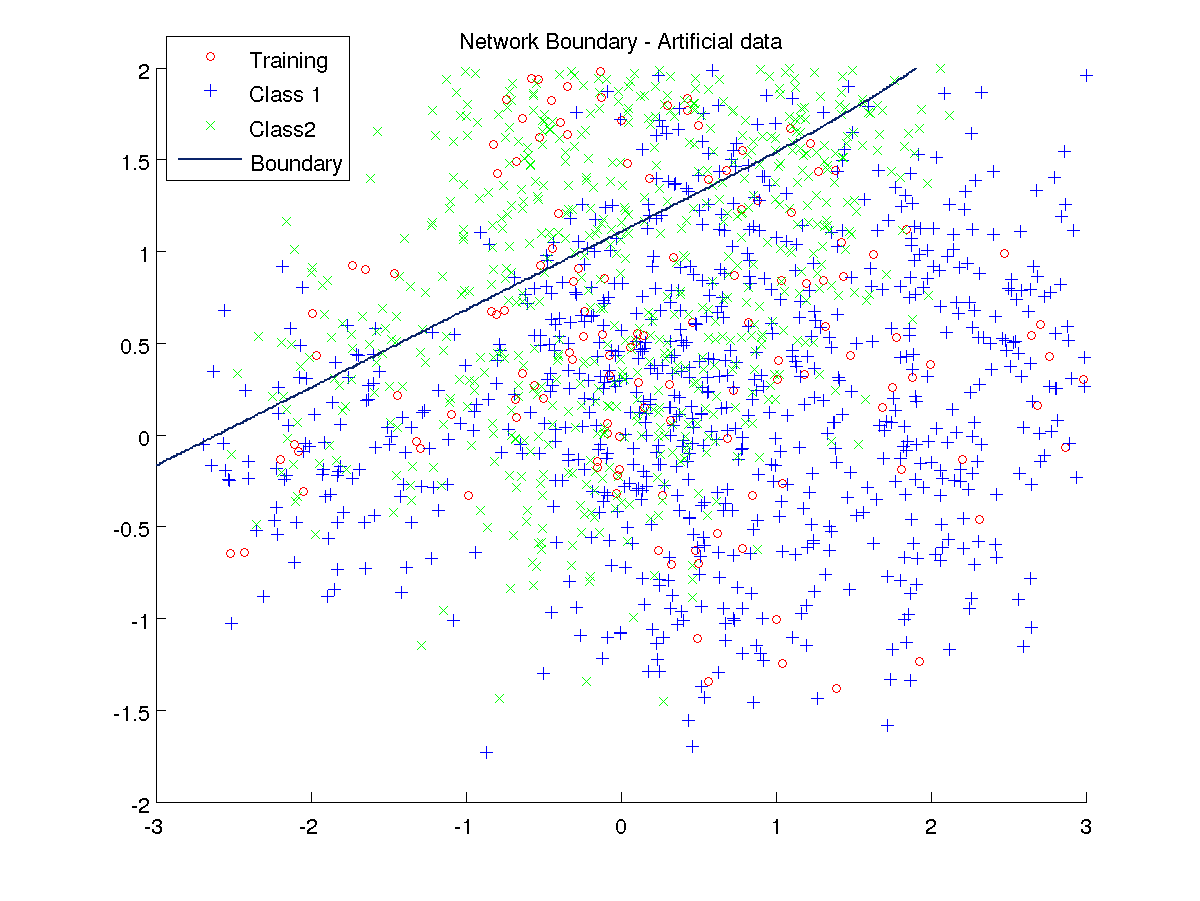
\includegraphics[width=1.0\textwidth]{./images/q210a_Nh2}
  \caption{}
  \label{fig:q210Nh2}
\end{figure}

\begin{figure}[!htbp]
  \centering
  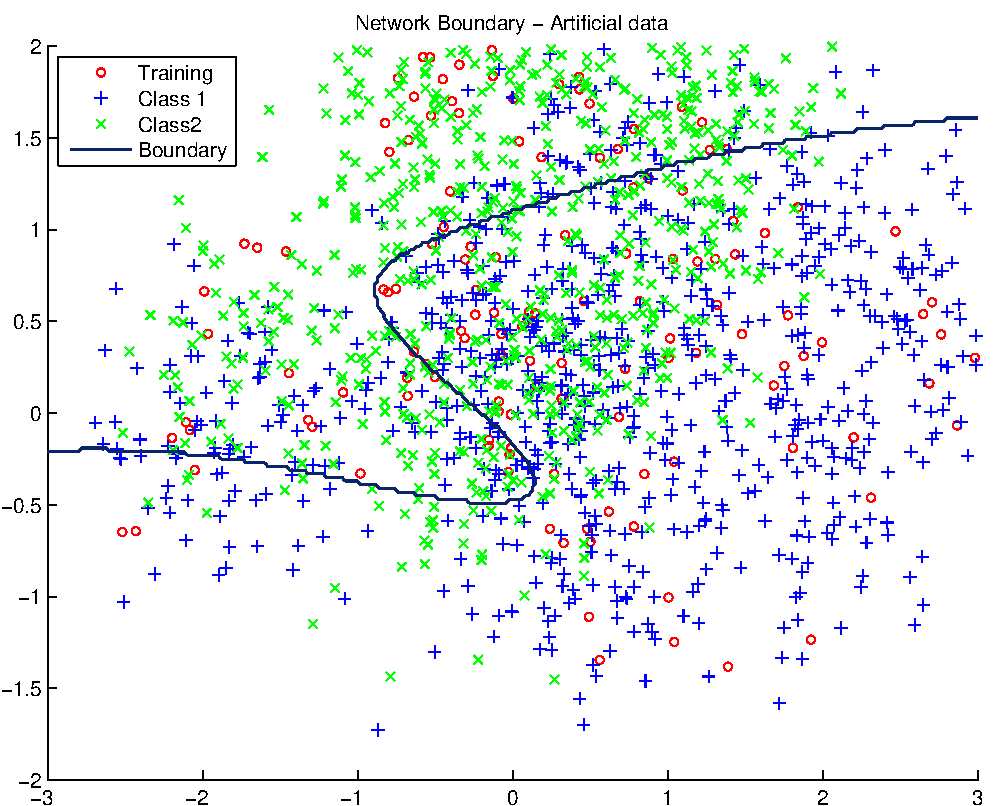
\includegraphics[width=1.0\textwidth]{./images/q210a_Nh260}
  \caption{}
  \label{fig:q210Nh260}
\end{figure}

\begin{figure}[!htbp]
  \centering
  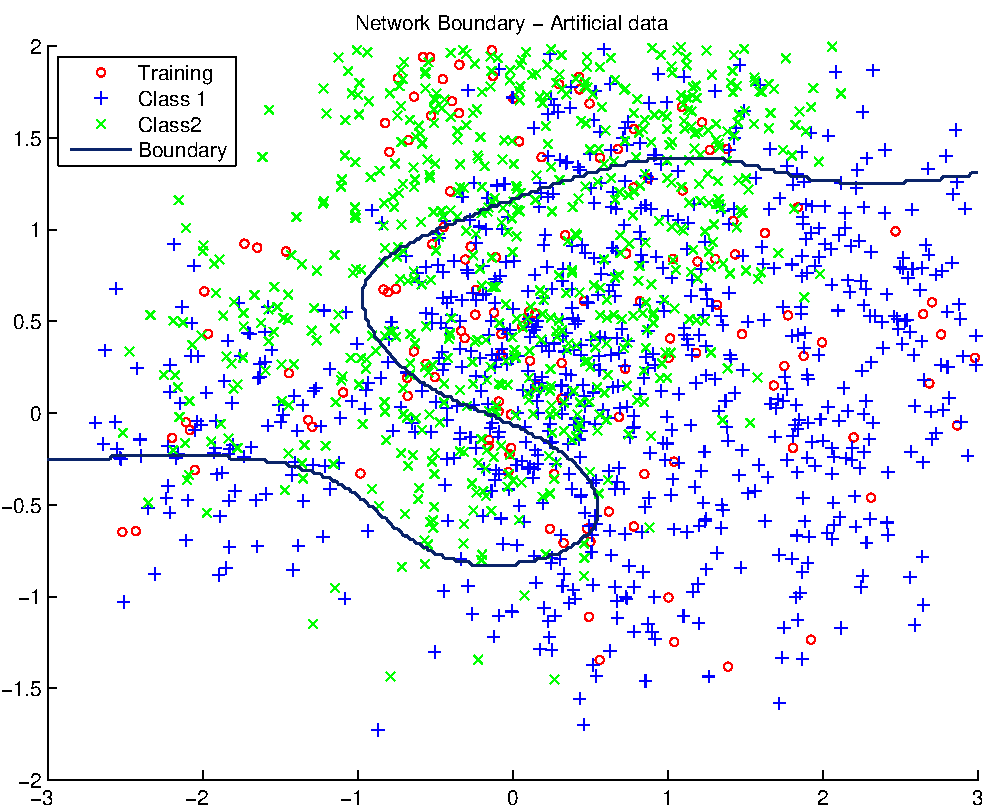
\includegraphics[width=1.0\textwidth]{./images/q210a_Nh1000}
  \caption{}
  \label{fig:q210Nh1000}
\end{figure}

In figure \ref{fig:q1_1} can be seen the $100$ data points drawn from
the gaussian distribution with $\mu = [1.0~ 1.0]$ and $\Sigma = [0.3~
  0.2; 0.2~ 0.2]$. The correct $\mu$ is blue and $\widehat{\mu}$ is
marked with red.

\begin{figure}[!htpb]
  \centering
%  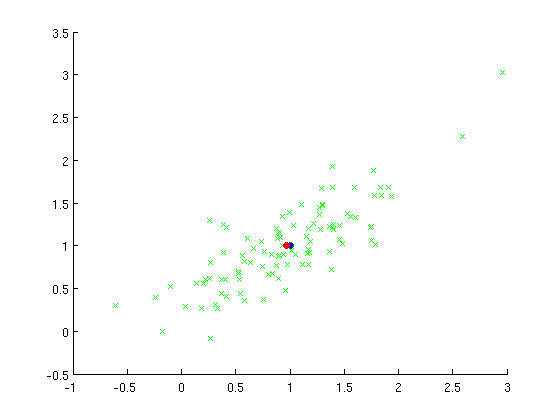
\includegraphics[width=0.6\textwidth]{images/q1_1}
  \caption{100 data points, correct mean with blue and estimated mean red.}
  \label{fig:q1_1}
\end{figure}

To quantify how much the estimated mean deviates from the correct
mean, we use usual euclidean distance between the two vectors.

Our distance is $0.0392$, which is not very much. This can also be
seen from the drawing, the points are placed really close.

The covariance matrix is also calculated on the training data:\\
$$\Sigma _{ML} = \left[
  \begin {array}{ccc}
    0.0082 & 0.0052 & 0.0067\\
    \noalign{\medskip}
    0.0052 & 0.0171 & 0.0199\\
    \noalign{\medskip}
    0.0067 & 0.0199 & 0.0241\\
  \end {array}
  \right]$$
% [0.0082~ 0.0052~ 0.0067; 0.0052~ 0.0171~ 0.0199; 0.0067~ 0.0199~ 0.0241]
